\section{The oriented diagram isotopy}\label{app:ports}

We prove Lemma~\ref{lem:isotopy} in the spherical braid projection.
The proof fixes the crossings of \(U\) and keeps track of the
two arcs where the new clasps are inserted.

\subsection{Port convention and initial cancellations}

A crossing has cyclic ports \(0,1,2,3\). The even pair is the
understrand and the odd pair the overstrand. A positive letter uses
inputs \((0,3)\) and outputs \((1,2)\) in left-to-right order.
A negative letter uses inputs \((1,0)\) and outputs \((2,3)\).
On each strand, connect its last output to its first input to close
the braid. Write \(\port{X}{j}\) for port \(j\) of crossing \(X\)
and take port indices modulo four.

Put \(r=b-4\) and number the crossings of \(Q'_bP_b\) from zero.
Cancel \(3b+3\) with \(5b\), followed by \(i\) with \(2r+13-i\)
for \(0\le i<r\), in increasing order. The first pair consists
of the two crossings in the circle detour. In each pair \((X,Z)\)
the bigon has edges \(\port X2\)--\(\port Z0\) and
\(\port X3\)--\(\port Z3\). The signs are opposite, with one branch
over at both crossings. These conditions specify Reidemeister II
cancellations.

The indexing of the uncancelled crossings and the neighbours
in the successive bigons can be obtained as follows. Name the
\(14\) crossings of \(U\) by \(F_j=r+j\). Use \(Y_i=2b+6+i\)
for the \(d-1\) crossings of \(\theta_d\), and set
\(u_j=3b+4+j,\ v_j=5b-1-j\) for \(0\le j<d\), the crossings
on the descending and returning parts of \(P_b\). The detour
cancellation connects \(\port{0}{3}\) to \(\port{(2b+5)}{3}\)
and \(\port{u_0}{3}\) to \(\port{v_0}{2}\). In the resulting
first bigon and at each later step \(i\), the four outside
neighbours of \(X=i,\ Z=2b+5-i\) are
\[
\begin{array}{c|l}
 \port X0&\port{v_i}1\\
 \port X1&\port{(i+1)}3\quad\text{if }i<r-1,\quad
                 \port{F_2}0\quad\text{if }i=r-1\\
 \port Z1&\port{(Z-1)}3\\
 \port Z2&\port{Y_{r-i}}3 .
\end{array}
\]
The cancellation connects \(\port{v_i}1\) to
\(\port{Y_{r-i}}3\) and wires the next bigon, with the last
step joining \(\port{F_2}0\) to \(\port{F_{13}}3\).
This describes the cancellations by induction. The listed
neighbours are obtained from the port rule by following the
consecutive crossings of \(\rho_b^{-1}\theta_d\) and the return
of \(P_b\). In particular the pairs use no crossing from \(U\).

Let \(A=\port{F_{12}}1,\ B=\port{F_{13}}2,\
C=\port{F_0}3,\ E=\port{F_1}3\). The edges of the remaining
diagram outside \(U\) are specified by their port neighbours
in Table~\ref{tab:ladder}. The \(Y_i\)'s follow the consecutive
crossings of \(\theta_d\), with \(\port{Y_i}2\) proceeding to
\(\port{Y_{i+1}}0\), or to \(\port{u_0}0\) at the end.
The two circuits past the circle follow the \(u_j\)'s in order
and the \(v_j\)'s in reverse order. At the doubled \(\sigma_2\)
the two crossings \(u_{d-1}\) and \(v_{d-1}\) meet directly.
The \(r\) joins from the cancelled bigons give the attachments
from \(v_i\) to \(Y_{r-i}\). With the four unchanged attachments
to \(U\) these traces give the table. All crossings in it are
positive.

\begin{table}[htbp]
\centering
\small
\begin{tabular}{@{}lcccc@{}}
\toprule
Crossing & Port \(0\) & Port \(1\) & Port \(2\) & Port \(3\)\\
\midrule
\(Y_0\) & \(A\) & \(\port{u_{d-1}}0\) & \(\port{Y_1}0\) & \(B\)\\
\(Y_i,\ 1\le i\le d-2\)
 & \(\port{Y_{i-1}}2\) & \(\port{u_{d-1-i}}0\)
 & \(\port{Y_{i+1}}0\) or \(\port{u_0}0\) & \(\port{v_{d-2-i}}1\)\\
\(u_0\)& \(\port{Y_{d-2}}2\)& \(\port{u_1}3\)&\(\port{v_0}3\)&\(\port{v_0}2\)\\
\(u_j,\ 1\le j\le d-2\)&\(\port{Y_{d-1-j}}1\)&\(\port{u_{j+1}}3\)
 &\(\port{v_j}3\)&\(\port{u_{j-1}}1\)\\
\(u_{d-1}\)&\(\port{Y_0}1\)&\(\port{v_{d-1}}0\)
 &\(\port{v_{d-1}}3\)&\(\port{u_{d-2}}1\)\\
\(v_0\)&\(\port{v_1}2\)&\(\port{Y_{d-2}}3\)&\(\port{u_0}3\)&\(\port{u_0}2\)\\
\(v_j,\ 1\le j\le d-3\)&\(\port{v_{j+1}}2\)&\(\port{Y_{d-2-j}}3\)
 &\(\port{v_{j-1}}0\)&\(\port{u_j}2\)\\
\(v_{d-2}\)&\(\port{v_{d-1}}2\)&\(E\)&\(\port{v_{d-3}}0\)&\(\port{u_{d-2}}2\)\\
\(v_{d-1}\)&\(\port{u_{d-1}}1\)&\(C\)&\(\port{v_{d-2}}0\)&\(\port{u_{d-1}}2\)\\
\bottomrule
\end{tabular}
\caption{Port neighbours after the initial cancellations.
The \(Y_i\) port \(2\) neighbour is \(\port{u_0}0\) at
\(i=d-2\). Every edge is reciprocal, including the ones meeting \(U\).}
\label{tab:ladder}
\end{table}

\subsection{Two local moves and the induction}

Write \((X,a),(Y,c),(Z,e)\) for the triangle with edges
\[
 \port{X}{(a+1)}\text{--}\port Yc,\qquad
 \port{Y}{(c+1)}\text{--}\port Ze,\qquad
 \port{Z}{(e+1)}\text{--}\port Xa .
\]
Consecutive ports make this a face in the oriented spherical
rotation system. The projection is connected and these faces
are empty disks. For the Reidemeister III moves below the
edges have respectively two underports, two overports, and
one of each. They are the bottom, top and middle branches
required for the move.

First consider the triangle \((u,3),(t,2),(v,1)\) with an
existing clasp attached, having edges
\(\port u1\)--\(\port w0\) and \(\port u2\)--\(\port w3\).
Use the six external endpoints in the first row of the table
below, in the cyclic order \((e_0,e_1,e_4,e_5,e_3,e_2)\);
the inputs are \(e_0,e_2,e_3\).
Apply Reidemeister III, first at this triangle and then at
\((w,3),(v,2),(t,1)\). The clasp edges persist, and the other
internal edges become
\(\port w1\)--\(\port t0,\ \port w2\)--\(\port v0,\
\port t3\)--\(\port v1\).
Tracing the three strands between the six endpoints gives the second row:
\[
\begin{array}{c|cccccc}
 &e_0&e_1&e_2&e_3&e_4&e_5\\\hline
 \text{before}&\port t0&\port t1&\port v0&\port v3&\port w1&\port w2\\
 \text{after}&\port u0&\port t1&\port u3&\port v3&\port t2&\port v2 .
\end{array}
\]
Thus the triangle can pass one clasp relative to all six
external endpoints.

For the same triangle at the cap (Figure~\ref{fig:cap}), use the extra edge
\(\port u2\)--\(\port v3\) and the first row below. The boundary
order is \((e_0,e_1,e_2,e_3)\), with inputs \(e_0,e_3\).
The same first Reidemeister III move creates a monogon
\(\port t2\)--\(\port t3\). Remove it by Reidemeister I.
The two crossings left form a positive clasp with edges
\(\port u1\)--\(\port v0,\ \port u2\)--\(\port v3\)
and the external attachments in the second row:
\[
\begin{array}{c|cccc}
 &e_0&e_1&e_2&e_3\\\hline
 \text{before}&\port t0&\port t1&\port u1&\port v0\\
 \text{after}&\port u0&\port v1&\port v2&\port u3 .
\end{array}
\]
In particular this is an ordinary positive full twist between
the two incoming strands. Both local rewrites keep the cyclic
boundary orders and orientations.


\begin{figure}[htbp]
\centering
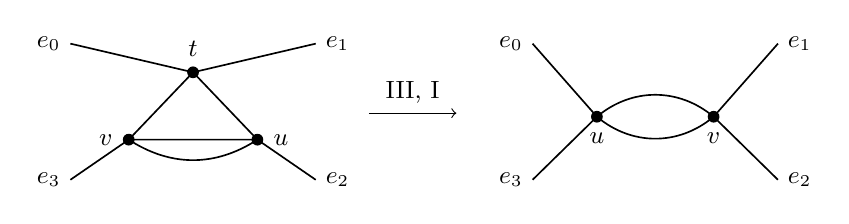
\begin{tikzpicture}[
    x=0.95cm,y=0.91cm,
    vertex/.style={circle,fill=black,inner sep=1.5pt},
    every node/.style={font=\small},
]
\begin{scope}[local bounding box=before]
  \coordinate (t) at (0,0.62);
  \coordinate (u) at (0.86,-0.32);
  \coordinate (v) at (-0.86,-0.32);
  \draw[semithick] (-1.64,1.02) node[left] {$e_0$} -- (t)
      -- (1.64,1.02) node[right] {$e_1$};
  \draw[semithick] (t) -- (v) -- (u) -- cycle;
  \draw[semithick] (v) to[bend right=33] (u);
  \draw[semithick] (-1.64,-0.88) node[left] {$e_3$} -- (v)
      (u) -- (1.64,-0.88) node[right] {$e_2$};
  \node[vertex,label=above:$t$] at (t) {};
  \node[vertex,label=right:$u$] at (u) {};
  \node[vertex,label=left:$v$] at (v) {};
\end{scope}
\draw[->] (2.35,0.05) -- node[above] {III, I} (3.52,0.05);
\begin{scope}[xshift=5.87cm]
  \coordinate (u) at (-0.78,0);
  \coordinate (v) at (0.78,0);
  \draw[semithick] (-1.64,1.02) node[left] {$e_0$} -- (u)
      -- (-1.64,-0.88) node[left] {$e_3$};
  \draw[semithick] (u) to[bend left=40] (v)
                   (u) to[bend right=40] (v);
  \draw[semithick] (1.64,1.02) node[right] {$e_1$} -- (v)
      -- (1.64,-0.88) node[right] {$e_2$};
  \node[vertex,label=below:$u$] at (u) {};
  \node[vertex,label=below:$v$] at (v) {};
\end{scope}
\end{tikzpicture}
\caption{The cap move viewed as a graph of crossings. The triangle
and cap on the left become a clasp on the right while the four
endpoints remain fixed. The port conventions specify the
overstrands and orientations.}
\label{fig:cap}
\end{figure}

Now put \(q=d-3\). At stage \(s\), for \(0\le s<q\), set
\(t=Y_{d-2-s}\). There are already \(s\) clasp pairs
\((u_j,v_j)\) for \(j<s\). Each has its two clasp edges, and
\[
       \port{v_j}1\text{--}\port{u_{j+1}}0,\qquad
       \port{v_j}2\text{--}\port{u_{j+1}}3 .
\]
The moving triangle begins at \((u_0,3),(t,2),(v_s,1)\).
At \(s=0\) the triangle and cap are in Table~\ref{tab:ladder}.
At each \(u_j\) for \(j<s\), use the first local rewrite
with \(w=v_j,\ v=v_s\). The two former attachments of \(w\)
to \(u_{j+1}\) now attach \(\port t2\) and \(\port{v_s}2\)
to \(u_{j+1}\), giving the triangle at \(u_{j+1}\).
This leaves \(\port{u_s}2\)--\(\port{v_s}3\) in place.
At \(u_s\), the cap rewrite removes \(t\) and gives the
clasp \((u_s,v_s)\).

To see the next stage, track the four ends of the unchanged
part of the ladder. At the start of stage \(s\),
\(\port t0\) is attached to \(\port{Y_{d-3-s}}2\)
and \(\port{v_s}0\) to \(\port{v_{s+1}}2\).
The first rewrite sends those attachments to \(\port{u_0}0\)
and \(\port{u_0}3\), whether it is at a clasp or at the cap.
Later moves in the stage keep them there. The cap rewires
\(\port t1\)--\(\port{u_{s+1}}0\) and
\(\port{u_s}1\)--\(\port{u_{s+1}}3\)
to the two new edges from \(\port{v_s}1,\port{v_s}2\).
The next triangle and cap therefore satisfy the same
hypotheses. This proves the induction for every \(d\).

At its end \(Y_2,\ldots,Y_{d-2}\) have been deleted.
The diagram consists of the \(d=3\) ladder with indices
\(Y_0,Y_1\) and \(u_q,u_{q+1},u_{q+2},v_q,v_{q+1},v_{q+2}\),
and \(q\) clasp pairs inserted between the two arcs
\(\port{Y_1}2\)--\(\port{u_q}0\) and
\(\port{v_q}2\)--\(\port{u_q}3\).
The first endpoint of each arc now leads into the first clasp (or directly to \(u_q\) if \(q=0\)). The two edges
from \(v_j\) to \(u_{j+1}\) then lead to the next clasp or
to the base ladder. All other edges of the base ladder remain
as specified in the table, and the crossings of \(U\) are fixed.

\subsection{Identifying the insertion band in \texorpdfstring{\(R\)}{R}}

Number the crossings of the literal word \(R\) from zero.
Its fourth and fifth closure arcs run from \(\port{24}2\)
to \(\port 00\) and from \(\port{25}1\) to \(\port 03\).
Cut those two arcs just before crossing zero, leaving a named
incoming and outgoing end for each arc. The Reidemeister II
pairs \((6,25)\) and \((7,22)\) cancel with the four ends
open. For the first pair the bigon edges are
\(\port 60\)--\(\port{25}2,\ \port 63\)--\(\port{25}3\).
For the second they are
\(\port 72\)--\(\port{22}0,\ \port 73\)--\(\port{22}3\)
after the first cancellation. The two incoming ends and
the fourth outgoing end stay attached to their ports.
The fifth outgoing end moves from \(\port{25}1\) to
\(\port 52\). Neither cancellation meets the slab at the cut.
The resulting \(22\)-crossing projection, with the arcs
reclosed, is the \(d=3\) ladder. The port bijection has no
rotations and is given by
\[
 \begin{array}{c|ccccccccc}
 &F_j&Y_0&Y_1&u_0&u_1&u_2&v_0&v_1&v_2\\\hline
 \text{crossing of }R&8+j&23&24&0&1&2&5&4&3 .
 \end{array}
\]
This is verified by the braid port rule, including the edges
of \(U\) and the four attachments in Table~\ref{tab:ladder}.
The cut arcs correspond precisely to
\(\port{Y_1}2\)--\(\port{u_0}0\) and
\(\port{v_0}2\)--\(\port{u_0}3\).
The marked ends identify the actual fourth/fifth strand band
before the first crossing of \(R\), including both boundary
orientations. In the closed braid a positive full twist in
that band can be written at the end of \(R\).
Each clasp from the induction has the port pairing of
\(\sigma_4^2\) in this band, so the resulting projection is
the twice-reduced diagram of \(\cl{R\sigma_4^{2q}}\).
The oriented moves preserve the component containing \(U\)
and the other component. Since \(q=b-5\), this proves
Lemma~\ref{lem:isotopy}.
